\documentclass[12pt]{article}
\usepackage{amsmath, amsthm, amssymb, enumerate, mathrsfs, graphicx, subfig, verbatim, float, pdflscape, rotating, parskip, setspace, tikz, tikz-qtree, url, epstopdf, mathtools, latexsym, flexisym, physics,accents, multirow,diagbox,accents}
\usepackage[framed,numbered,autolinebreaks,useliterate]{mcode}
\usepackage{url}
\usepackage{listings}
\usepackage{pdfpages}
\usepackage{breqn}

\usepackage[margin=1in]{geometry}
\usepackage[round]{natbib}
\addtolength{\parskip}{\baselineskip}
\DeclareMathSizes{12}{13}{7}{7}
\usepackage[bottom]{footmisc}
\newcommand{\ubar}[1]{\underaccent{\bar}{#1}}

\parskip 2pt
\setlength\parindent{0cm}
\begin{document}
\begin{onehalfspace}


\title{Econ 8307\\ Assignment 1 (Spring 2019)}
\author{Jonah Coste, Fred Xu\\George Washington University}
\date{}
\maketitle
\parskip 10pt
\textbf{Question 1}\\
\begin{enumerate}[(a)]
	\item
	\begin{enumerate}[1.]
\item
returns a pseudorandom scalar integer N between 1 and 10
\begin{lstlisting}
N = randi(10);
\end{lstlisting}
\item
Generating a vector of N real numbers, where each value is drawn from the uniform distribution over [-1;1]. Expected value of mean is 0.
\begin{lstlisting}
X = rand(N,1)*2 -1;
\end{lstlisting}
\item
\begin{enumerate}[3.1]
	\item
	Computing the mean of the N real numbers using loops
	\begin{lstlisting}
sum1 = 0;
for i=1:N
	sum1 = sum1 + X(i);
end
result1 = sum1/N;
	\end{lstlisting}
	\item
	Computing the mean of the N real numbers using Matlab built-in function
	\begin{lstlisting}
result2 = mean(X);
	\end{lstlisting}
\end{enumerate}
\item
Printing both results
\begin{lstlisting}
 result1
 result2

result1 =

    0.0111


result2 =

    0.0111
\end{lstlisting}
	\end{enumerate}
	\item
	\begin{enumerate}[1.]
\item
Generating three random positive integers N, M and L
\begin{lstlisting}
N = randi(10);
M = randi(10);
L = randi(10);
\end{lstlisting}
\item
Generating a $NxM$ matrix of real numbers as before, and also a $MxL$ matrix
\begin{lstlisting}
matrix1 = rand(N,M)*2 -1;
matrix2 = rand(M,L)*2 -1;
\end{lstlisting}
\item
\begin{enumerate}[3.1]
	\item
	Multiplying matrix 1 and matrix 2 using loops
	\begin{lstlisting}
resultmatrix1 = zeros(N,L);
for i =1:N
	for j = 1:L  
val = 0;
for h = 1:M
	val = val + matrix1(i,h) * matrix2(h,j);
end
resultmatrix1(i,j) = val;
	end
end
	\end{lstlisting}
	\item
	Multiplying matrix 1 and matrix 2 using Matlab function
	\begin{lstlisting}
resultmatrix2 = matrix1 * matrix2;
	\end{lstlisting}
\end{enumerate}
\item
Printing both results
\begin{lstlisting}
 resultmatrix1
 resultmatrix2

resultmatrix1 =

   -1.3531    0.7949    1.2546    0.7810    1.6366   -0.7368
    1.0276   -1.9193   -0.8117   -0.9999   -1.9131    0.5385
   -0.0565   -1.8597   -0.2167   -0.9230    0.0832    0.3726
   -0.4876    0.0426    0.2310   -0.1071   -0.1139   -0.7056
    0.2503    0.1662   -1.0685   -0.1601   -0.3765   -0.2254
    0.9476    0.8543   -0.8032   -0.0655   -0.5442    0.7607
   -0.9518   -0.5732    0.6697    0.2639    0.2710   -0.5262
   -0.6902    0.0980    1.2289    0.5333    1.1795    0.8939
    0.3438    0.7926    0.3158    0.4998   -0.1655   -0.8317


resultmatrix2 =

   -1.3531    0.7949    1.2546    0.7810    1.6366   -0.7368
    1.0276   -1.9193   -0.8117   -0.9999   -1.9131    0.5385
   -0.0565   -1.8597   -0.2167   -0.9230    0.0832    0.3726
   -0.4876    0.0426    0.2310   -0.1071   -0.1139   -0.7056
    0.2503    0.1662   -1.0685   -0.1601   -0.3765   -0.2254
    0.9476    0.8543   -0.8032   -0.0655   -0.5442    0.7607
   -0.9518   -0.5732    0.6697    0.2639    0.2710   -0.5262
   -0.6902    0.0980    1.2289    0.5333    1.1795    0.8939
    0.3438    0.7926    0.3158    0.4998   -0.1655   -0.8317

\end{lstlisting}
	\end{enumerate}
\end{enumerate}

\textbf{Question 2}\\
\begin{enumerate}[(a)]
	\item
	Use World Bank Indicator data for GDP per capita in constant 2010 US\$ for China and USA for years 1960-2017 available here \url{https://data.worldbank.org/indicator/NY.GDP.PCAP.KD?locations=CN-US}
	\item
	Load GDP per capita data into Matlab as vectors.
	\begin{lstlisting}
China = [191.791179910216;..;7329.08929913216];
USA = [17036.8851695882;..;53128.5396999252];
	\end{lstlisting}
	\item
	Computing GDP per capita growth rate and plotting over time
	\begin{lstlisting}
sz = size(China,1) - 1;
Growth = zeros(sz ,2);
Year = zeros(sz,1);
for i = 1:sz
	Growth(i,1) = China(i+1,1) / China(i,1) -1;
	Growth(i,2) = USA(i+1,1) / USA(i,1) -1;
	Year(i,1) = 1960 + i;
end
figure
plot(Year, Growth)
title('Real GDP Per Capita Growth Rate for China and USA 1961-2017')
xlabel('Year')
ylabel('Growth Rate')
legend({'China','USA'},'Location','southeast')
	\end{lstlisting}
	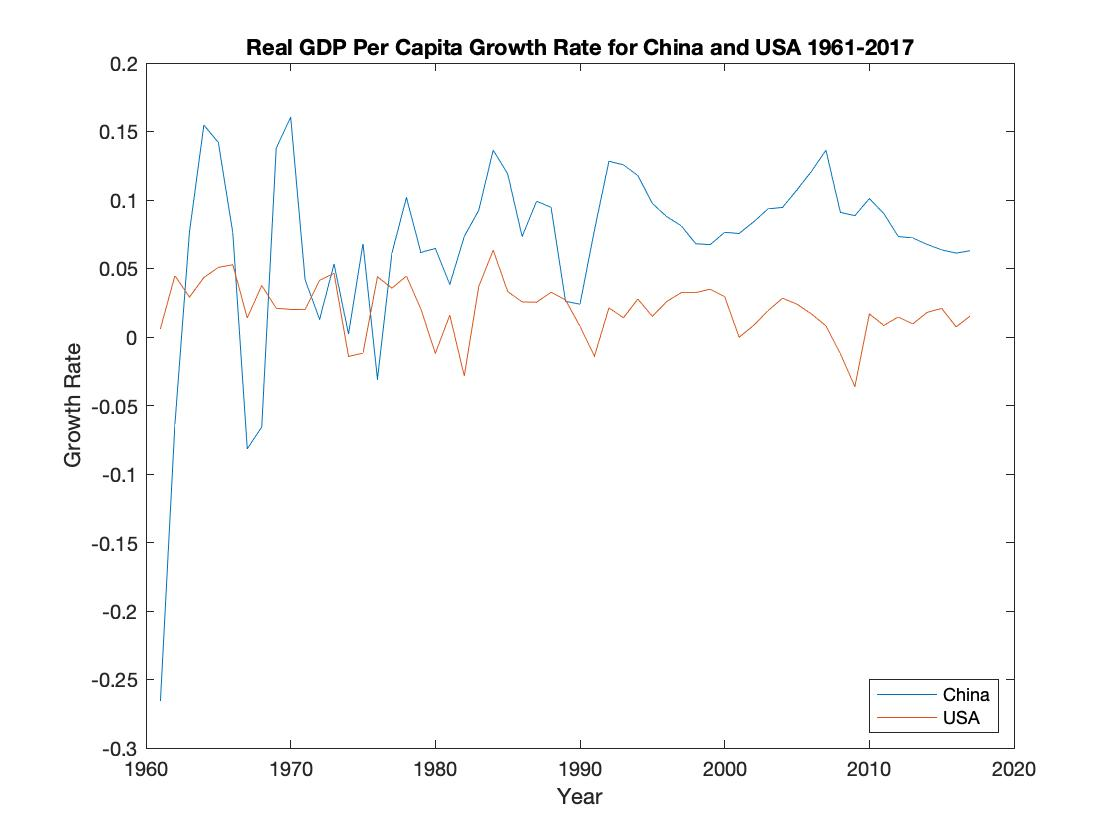
\includegraphics[width=\textwidth]{Econ_8307_PS1.jpg}
\end{enumerate}

\textbf{Question 3}

\begin{enumerate}[(a)]
	\item
	Agent's budget constraint is:
	\begin{equation}
\begin{split}
f(k_t) + (1-\delta) * k_t &>= c_t + k_{t+1}\\
k_{t+1} &>= 0
\end{split}
	\end{equation}
	\item
	From t=1 to T-1 the first order condition that charachterizes the solution is:
	\begin{equation}
	u^\prime(c_t) = \beta * u^\prime(c_{t+1}) * [f^\prime(k_{t+1}) + 1 - \delta]
	\end{equation}
	The optimality condtion at period T is:
	\begin{equation}
	c_T =  f(k_T) + (1-delta) * k_T
	\end{equation}
	At the end of period T there should be zero capital left over
	\begin{equation}
	k_{T+1} = 0
	\end{equation}
	\item
	Finding the solution numerically
	\begin{lstlisting}
%parameters
beta = .97;
delta = .1;
theta = .3;
T = 4;
epsilon=1e-15;
initialcapital = 1;
guessinitialcons = initialcapital; %could be any guess

if guessinitialcons < 0
guessinitialcons = 0;
end %fail safe

c = zeros(T,1);
k = zeros (T+1,1);
k(1) = initialcapital;

guess = guessinitialcons;
last = -2*epsilon; % to allow for guess of 0
step = k(1);

while abs(guess - last) > epsilon || abs(k(T+1)) > epsilon
c(1) = guess;
ind = 0;
for i= 1: T-1
   if k(i)^theta + (1 - delta)*k(i) - c(i) >= 0
   k(i+1) = k(i)^theta + (1 - delta)*k(i) - c(i);
   c(i+1) = beta * c(i) * (theta * k(i+1)^(theta-1) + 1 - delta);
   else
   ind = 1;
   end
end
k(T+1) = k(T)^theta + (1 - delta)*k(T) - c(T);
if k(T+1) < 0 || ind == 1
step = step/2;
guess = last + step;
else
last = guess;
guess = guess + step;
end
end

%Print optimal consumption and capital series
c
k

c =

    0.8629
    0.9980
    1.1731
    1.4797


k =

    1.0000
    1.0371
    0.9464
    0.6622
   -0.0000
\end{lstlisting}
We have set the tolerance level equal to epsilon (initally $10^{-15}$). This means our answer, while approximate, will have leftover capital of less than epsilon in absolute value. Each period's consumption is therefore at least that "close" to the actual optimal vlaue.
\end{enumerate}



\end{onehalfspace}
\end{document}